% ==============================================================================
% INTRO SECTION
% Motivation, research design, and main result
% ==============================================================================

% ==============================================================================
% SLIDE 1
% ==============================================================================
\begin{frame}[t]
    \frametitle{Local land-use control creates a welfare tradeoff}
    \small

    \begin{columns}[T,totalwidth=\textwidth]
        \begin{column}{0.48\textwidth}
            \begin{block}{Why local control can be beneficial}
                \begin{itemize}
                    \item Local officials observe congestion and neighborhood costs.
                    \item Decentralization can screen out high-damage projects.
                \end{itemize}
            \end{block}
        \end{column}
        \begin{column}{0.5\textwidth}
            \begin{block}{Why local control can hurt}
                \begin{itemize}
                    \item Housing benefits spill across districts through rents, wages, and agglomeration.
                    \item Incumbent homeowners may block projects with benefits elsewhere.
                \end{itemize}
            \end{block}
        \end{column}
    \end{columns}
    
    \vspace{0.02em}
    \begin{center}
        \begin{minipage}{0.88\textwidth}
            \centering
            \textbf{Question:} How does shifting land-use authority to local districts affect housing supply and welfare across the city?
        \end{minipage}
    \end{center}

    \vspace{0.02em}
    \noindent
    \begin{minipage}{0.94\textwidth}
        \raggedright
        {\large\bfseries This paper}\par
        \vspace{0.35em}
        \footnotesize
        After NYC shifts land-use authority toward district-based control,
        large multifamily production shifts away from homeowner-heavy districts.
        I plan to map this reduced-form evidence into a quantitative spatial model
        with an institution-dependent land-use approval stage, where centralized
        and decentralized regimes differ in how they weigh citywide spillovers,
        local information, and incumbent political pressure.
    \end{minipage}

\end{frame}

% ==============================================================================
% SLIDE 2
% ==============================================================================
\begin{frame}
    \frametitle{Local control is a hot topic among policymakers and academics}
    \begin{minipage}{0.5\textwidth}
        \begin{figure}
            \centering
            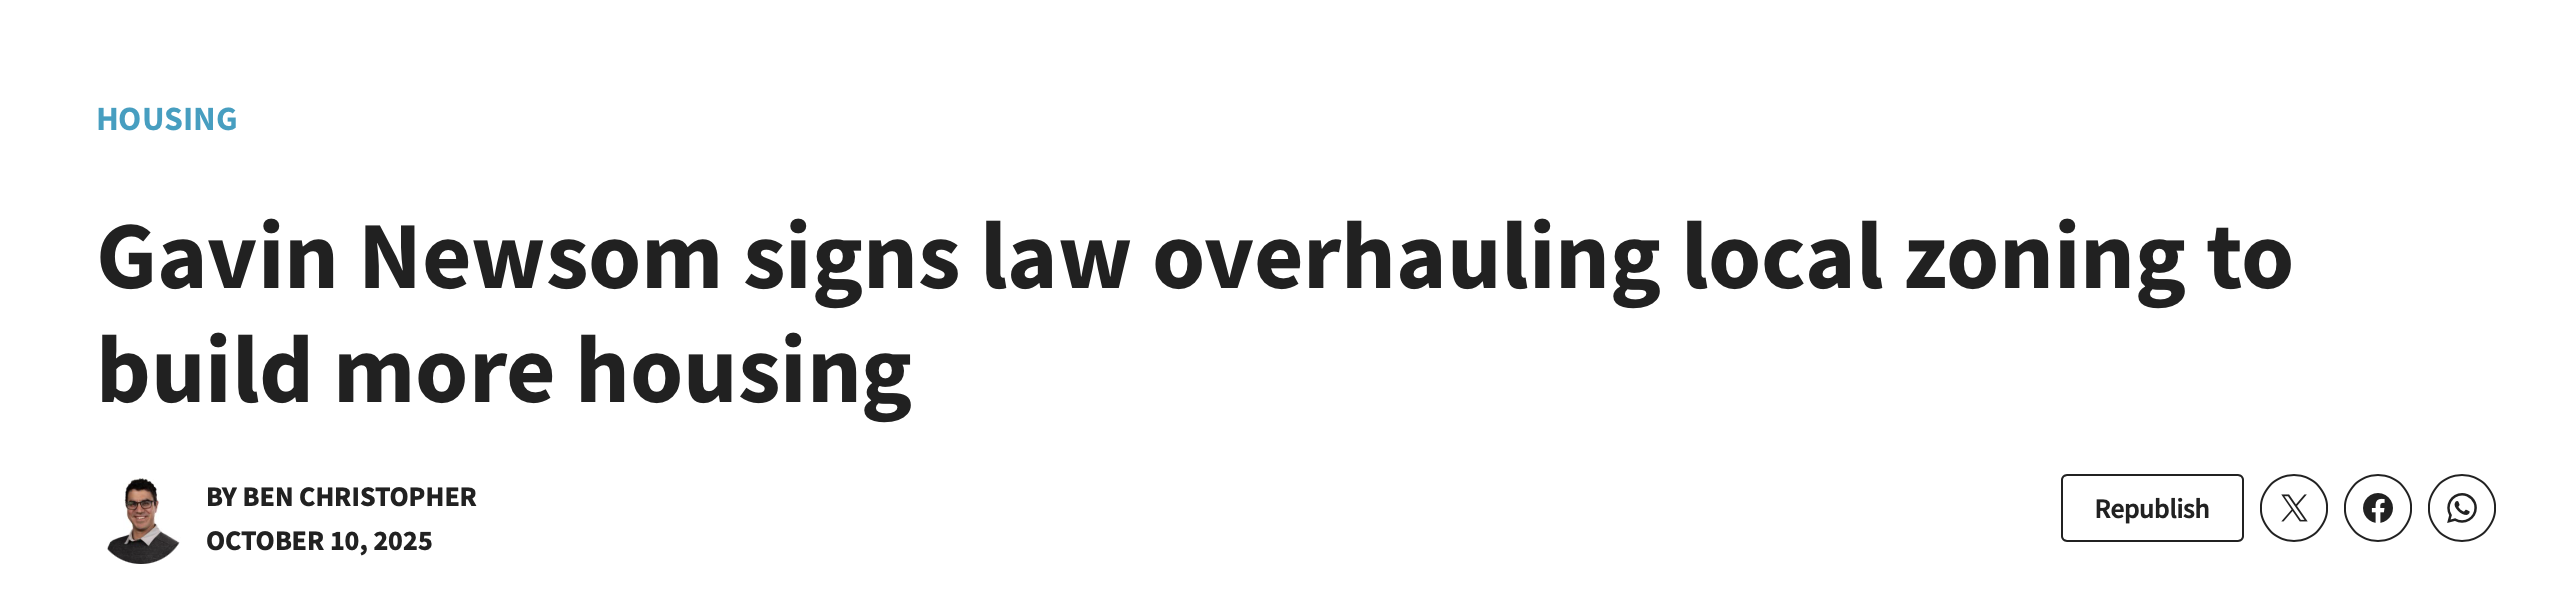
\includegraphics[width=\textwidth]{images/california_local_control.png}
        \end{figure}
        \begin{figure}
            \centering
            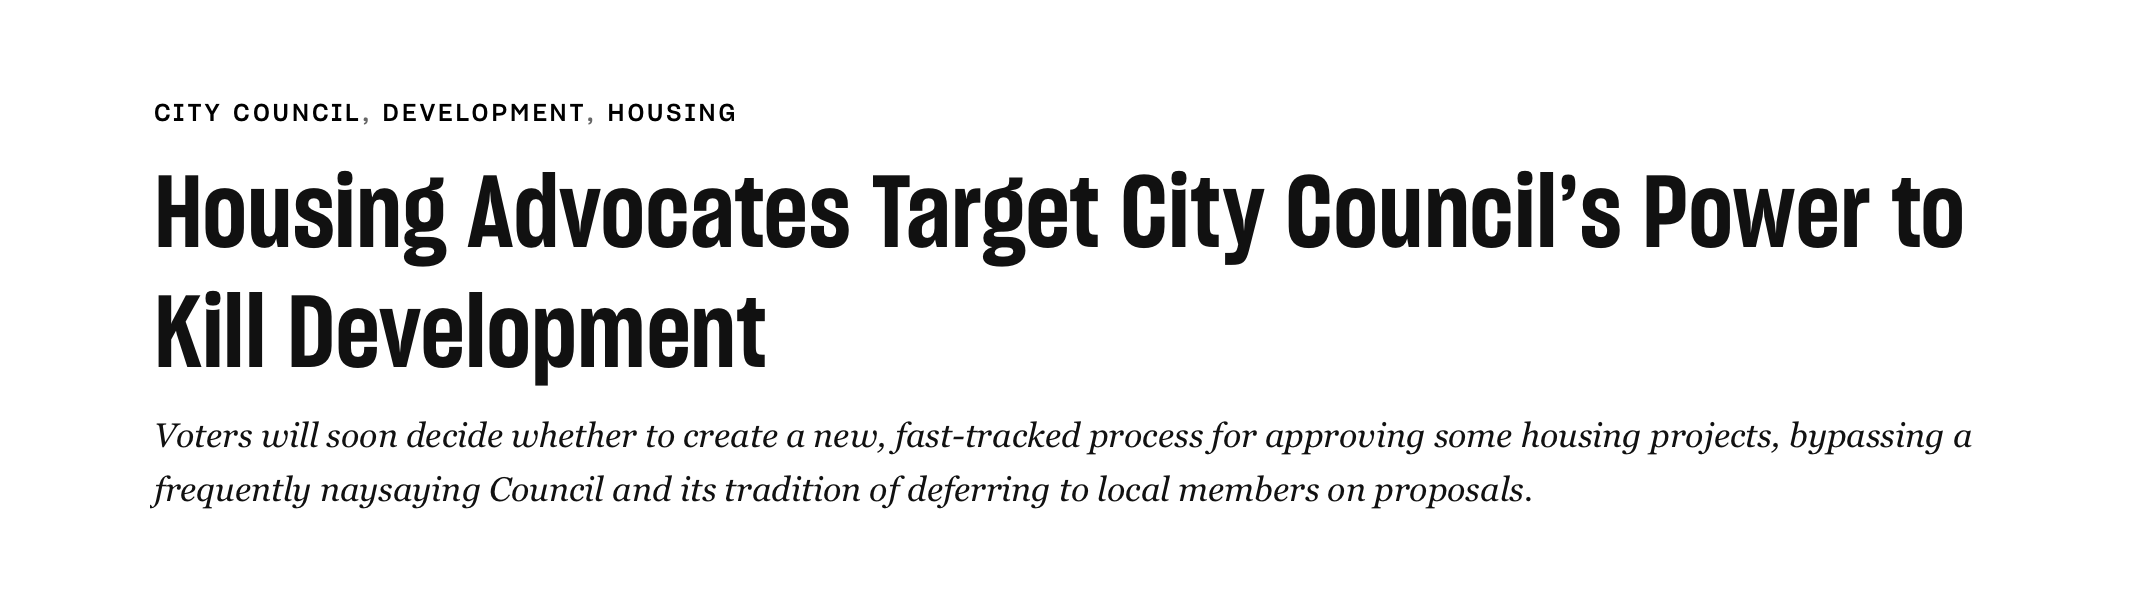
\includegraphics[width=\textwidth]{images/nyc_member_deference.png}
        \end{figure}
        \begin{figure}
            \centering
            
\includegraphics[width=\textwidth]{images/illinois_local_control_pritzker.png}
        \end{figure}
    \end{minipage}
    \hfill
    \begin{minipage}{0.48\textwidth}
        \begin{figure}
            \centering
            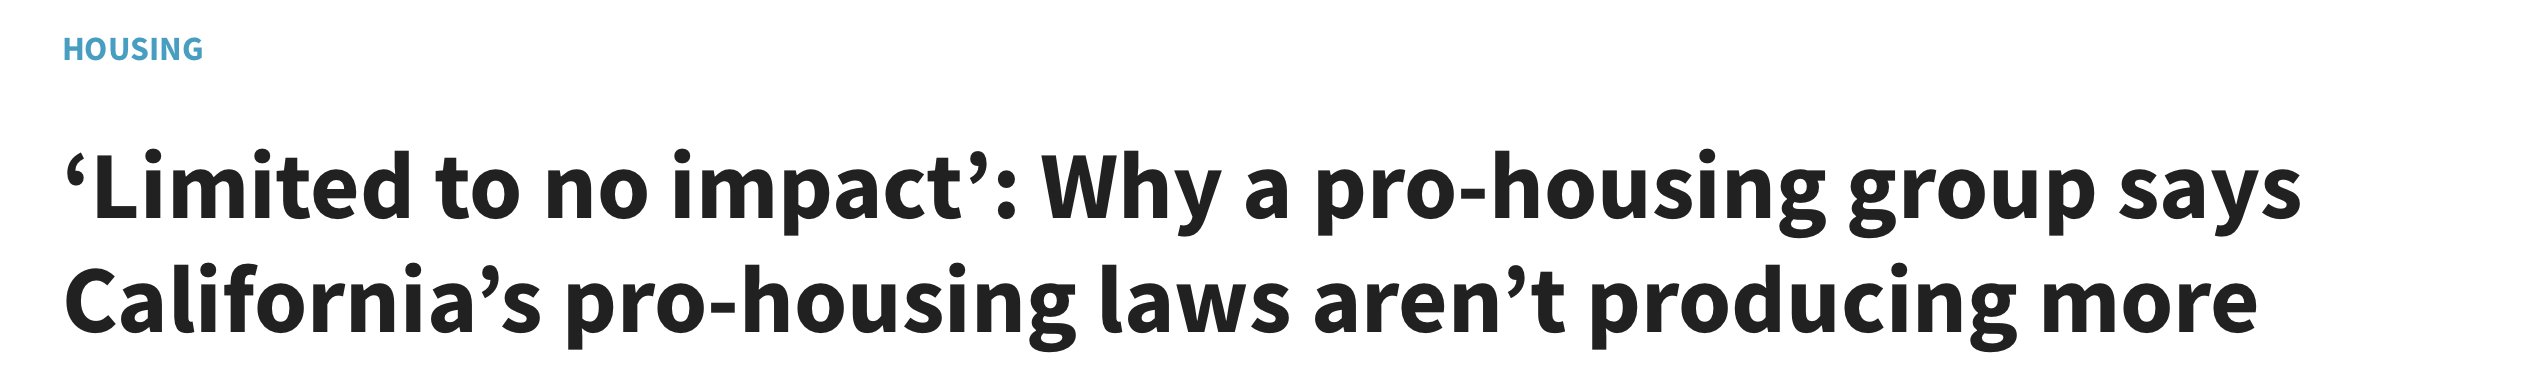
\includegraphics[width=\textwidth]{images/california_ineffective.png}
        \end{figure}
        \begin{figure}
            \centering
            
\includegraphics[width=\textwidth]{images/local_control_good_noah_smith.png}
        \end{figure}
    \end{minipage}
\end{frame}

\newcommand{\ClassInstitutionalTimelineSetup}{%
    \definecolor{timelineblue}{HTML}{3366CC}%
    \definecolor{timelinegray}{HTML}{777777}%
    \definecolor{timelinered}{HTML}{CC3311}%
    \definecolor{timelinegold}{HTML}{D99A20}%
    \definecolor{timelinegreen}{HTML}{238B45}%
    \definecolor{timelinedark}{HTML}{30343B}%
    \pgfplotsset{
        institutional timeline axis/.style={
            width=0.97\textwidth,
            height=0.68\textheight,
            xmin=1980,
            xmax=2025,
            ymin=0.07,
            ymax=0.70,
            clip=false,
            xlabel={Year},
            xlabel style={font=\scriptsize, yshift=-0.1em},
            xtick={1980,2002,2010,2025},
            xticklabel={\pgfmathprintnumber[fixed,precision=0,1000 sep={}]{\tick}},
            xticklabel style={font=\scriptsize},
            ytick={0.1,0.2,0.3,0.4,0.5},
            minor x tick num=1,
            minor y tick num=1,
            tick label style={font=\scriptsize},
            legend style={
                draw=none,
                font=\scriptsize,
                at={(0.60,-0.20)},
                anchor=north,
                legend columns=3
            },
            legend cell align=left,
        }
    }%
}

\newcommand{\ClassInstitutionalTimelinePieces}{%
    \draw[line width=2.8pt, draw=timelinedark!85]
        (axis cs:1980,0.086) -- (axis cs:2025,0.086);

    \path[fill=timelinedark!18, draw=timelinedark!45, rounded corners=1.1pt]
        (axis cs:1980,0.074) rectangle (axis cs:1989,0.103);
    \node[font=\tiny\bfseries, align=center, text width=1.45cm, text=timelinedark, anchor=north]
        at (axis cs:1984.25,0.026) {Board of\\Estimate};

    \path[fill=timelinegold!22, draw=timelinegold!65, rounded corners=1.1pt]
        (axis cs:1989,0.074) rectangle (axis cs:1991,0.103);
    \node[font=\tiny\bfseries, align=center, text width=1.05cm, text=timelinegold!55!black, anchor=north]
        at (axis cs:1989.95,0.026) {Morris\\Charter};

    \path[fill=timelineblue!12, draw=timelineblue!45, rounded corners=1.1pt]
        (axis cs:1991,0.074) rectangle (axis cs:2002,0.103);
    \node[font=\tiny\bfseries, align=center, text width=2.0cm, text=timelineblue!70!black, anchor=north]
        at (axis cs:1996.6,0.026) {New Council\\district map};

    \path[fill=timelinered!12, draw=timelinered!50, rounded corners=1.1pt]
        (axis cs:2002,0.074) rectangle (axis cs:2024,0.103);
    \node[font=\tiny\bfseries, align=center, text=timelinered!75!black, anchor=north]
        at (axis cs:2013,0.026) {Member deference\\era};

    \path[fill=timelinegreen!15, draw=timelinegreen!55, rounded corners=1.1pt]
        (axis cs:2024,0.074) rectangle (axis cs:2025,0.103);
    \node[font=\tiny\bfseries, align=center, text width=1.05cm, text=timelinegreen!55!black, anchor=north]
        at (axis cs:2023.85,0.026) {City\\of Yes};

    \draw[densely dashed, line width=0.7pt, draw=timelinegold!80!black]
        (axis cs:1989,0.105) -- (axis cs:1989,0.635);
    \node[font=\tiny, align=center, text width=1.95cm, fill=white, fill opacity=0.92, text opacity=1, rounded corners=2pt, inner sep=2pt, draw=timelinegold!55]
        at (axis cs:1985.85,0.660) {\textbf{1989}\\Supreme Court\\invalidates Board of Estimate};

    \draw[densely dashed, line width=0.7pt, draw=timelineblue!70!black]
        (axis cs:1991,0.105) -- (axis cs:1991,0.560);
    \node[font=\tiny, align=center, text width=1.75cm, fill=white, fill opacity=0.92, text opacity=1, rounded corners=2pt, inner sep=2pt, draw=timelineblue!45]
        at (axis cs:1994.65,0.585) {\textbf{1991}\\Districted\\Council begins};

    \draw[densely dashed, line width=0.7pt, draw=timelinered!80!black]
        (axis cs:2002,0.105) -- (axis cs:2002,0.635);
    \node[font=\scriptsize, align=center, text width=2.15cm, fill=white, fill opacity=0.90, text opacity=1, rounded corners=2pt, inner sep=2pt, draw=timelinered!45]
        at (axis cs:2004.6,0.660) {\textbf{2002}\\Vallone exits;\\deference hardens};

    \draw[densely dashed, line width=0.7pt, draw=timelinegreen!70!black]
        (axis cs:2025,0.105) -- (axis cs:2025,0.635);
    \node[font=\scriptsize, align=center, text width=2.0cm, fill=white, fill opacity=0.90, text opacity=1, rounded corners=2pt, inner sep=2pt, draw=timelinegreen!45]
        at (axis cs:2023.4,0.660) {\textbf{2025}\\reform\\frontier};
}

\newcommand{\ClassInstitutionalTimelinePiecesCounts}{%
    \draw[line width=2.8pt, draw=timelinedark!85]
        (axis cs:1980,560) -- (axis cs:2025,560);

    \path[fill=timelinedark!18, draw=timelinedark!45, rounded corners=1.1pt]
        (axis cs:1980,140) rectangle (axis cs:1989,1150);
    \node[font=\tiny\bfseries, align=center, text width=1.45cm, text=timelinedark, anchor=north]
        at (axis cs:1984.25,-1540) {Board of\\Estimate};

    \path[fill=timelinegold!22, draw=timelinegold!65, rounded corners=1.1pt]
        (axis cs:1989,140) rectangle (axis cs:1991,1150);
    \node[font=\tiny\bfseries, align=center, text width=1.05cm, text=timelinegold!55!black, anchor=north]
        at (axis cs:1989.95,-1540) {Morris\\Charter};

    \path[fill=timelineblue!12, draw=timelineblue!45, rounded corners=1.1pt]
        (axis cs:1991,140) rectangle (axis cs:2002,1150);
    \node[font=\tiny\bfseries, align=center, text width=2.0cm, text=timelineblue!70!black, anchor=north]
        at (axis cs:1996.6,-1540) {New Council\\district map};

    \path[fill=timelinered!12, draw=timelinered!50, rounded corners=1.1pt]
        (axis cs:2002,140) rectangle (axis cs:2024,1150);
    \node[font=\tiny\bfseries, align=center, text=timelinered!75!black, anchor=north]
        at (axis cs:2013,-1540) {Member deference\\era};

    \path[fill=timelinegreen!15, draw=timelinegreen!55, rounded corners=1.1pt]
        (axis cs:2024,140) rectangle (axis cs:2025,1150);
    \node[font=\tiny\bfseries, align=center, text width=1.05cm, text=timelinegreen!55!black, anchor=north]
        at (axis cs:2023.85,-1540) {City\\of Yes};

    \draw[densely dashed, line width=0.7pt, draw=timelinegold!80!black]
        (axis cs:1989,1220) -- (axis cs:1989,19750);
    \node[font=\tiny, align=center, text width=1.95cm, fill=white, fill opacity=0.92, text opacity=1, rounded corners=2pt, inner sep=2pt, draw=timelinegold!55]
        at (axis cs:1985.85,20600) {\textbf{1989}\\Supreme Court\\invalidates Board of Estimate};

    \draw[densely dashed, line width=0.7pt, draw=timelineblue!70!black]
        (axis cs:1991,1220) -- (axis cs:1991,17100);
    \node[font=\tiny, align=center, text width=1.75cm, fill=white, fill opacity=0.92, text opacity=1, rounded corners=2pt, inner sep=2pt, draw=timelineblue!45]
        at (axis cs:1994.65,18000) {\textbf{1991}\\Districted\\Council begins};

    \draw[densely dashed, line width=0.7pt, draw=timelinered!80!black]
        (axis cs:2002,1220) -- (axis cs:2002,19750);
    \node[font=\scriptsize, align=center, text width=2.15cm, fill=white, fill opacity=0.90, text opacity=1, rounded corners=2pt, inner sep=2pt, draw=timelinered!45]
        at (axis cs:2004.6,20600) {\textbf{2002}\\Vallone exits;\\deference hardens};

    \draw[densely dashed, line width=0.7pt, draw=timelinegreen!70!black]
        (axis cs:2025,1220) -- (axis cs:2025,19750);
    \node[font=\scriptsize, align=center, text width=2.0cm, fill=white, fill opacity=0.90, text opacity=1, rounded corners=2pt, inner sep=2pt, draw=timelinegreen!45]
        at (axis cs:2023.4,20600) {\textbf{2025}\\reform\\frontier};
}


% ==============================================================================
% SLIDE 2
% ==============================================================================
\begin{frame}[t,label=main-result-share]
    \frametitle{Institutional setting: New York City's shift to local control}
    \small

    \begin{columns}[T,totalwidth=\textwidth]
        \begin{column}{0.48\textwidth}
            \begin{block}{Before 1989: citywide/borough-scale review}
                \begin{itemize}
                    \item Board of Estimate held final authority over many land-use actions
                    \begin{itemize}
                        \item 11 votes total: 2 for mayor, 2 for comptroller, 2 for City Council President, and 1 for each borough president.
                    \end{itemize}
                    \item The 1989 Supreme Court decision \textit{Morris v. Board of Estimate} invalidated the Board's structure under the ``one person, one vote'' principle.
                \end{itemize}
            \end{block}
        \end{column}
        \begin{column}{0.48\textwidth}
            \begin{block}{After \textit{Morris}: district-based review}
                \begin{itemize}
                    \item The 1989 Charter revision process abolished the Board.
                    \item A 51-member City Council takes final legislative review.
                    \item Over time, ``member deference'' made district members pivotal for local land-use actions.
                \end{itemize}
            \end{block}
        \end{column}
    \end{columns}

\end{frame}

\begin{frame}[t]
    \frametitle{Measuring political exposure: 1990 homeownership by council district}
    \small

    \begin{columns}[T,totalwidth=\textwidth]
        \begin{column}{0.46\textwidth}
            \begin{itemize}
                \item Assign 1990 NHGIS tract tenure counts to 2010 Council districts
                \item Compute each district's owner-occupied share.
                \item Standardize within borough:
            \end{itemize}

            \vspace{-0.4em}
            \[
                T_j =
                \frac{h_j - \bar h_{b(j)}}{s_{b(j)}}.
            \]

            \begin{itemize}
                \item Positive values identify homeowner-heavy districts relative to nearby political peers.
            \end{itemize}
        \end{column}
        \begin{column}{0.50\textwidth}
            \vspace{-1.0em}
            \begin{center}
                \includegraphics[page=1,height=0.74\textheight,trim={0.25in 0in 0.25in 0in},clip]{../tasks/build_ccd2010_homeownership_1990_measure/output/ccdist2010_homeownership_1990_map.pdf}
            \end{center}
        \end{column}
    \end{columns}
\end{frame}

% ==============================================================================
% SLIDE 3
% ==============================================================================
\begin{frame}[t]
    \frametitle{Timeline of land-use authority in New York City}

    \begingroup
    \ClassInstitutionalTimelineSetup

    \centering
    \begin{tikzpicture}
    \begin{axis}[
        institutional timeline axis,
        axis lines=left,
        ylabel={Share of units built (3-year centered MA)},
        ylabel style={font=\scriptsize, opacity=0},
        yticklabel style={font=\scriptsize, opacity=0},
        ytick style={draw=none},
        y axis line style={draw=none},
        grid=none,
    ]
        \ClassInstitutionalTimelinePieces
    \end{axis}
    \end{tikzpicture}
    \endgroup
\end{frame}

% ==============================================================================
% SLIDE 4
% ==============================================================================
\begin{frame}[t]
    \frametitle{Main result: new units shift away from homeowner-heavy districts}

    \begingroup
    \ClassInstitutionalTimelineSetup

    \centering
    \begin{tikzpicture}
    \begin{axis}[
        institutional timeline axis,
        axis lines=left,
        xlabel={},
        ylabel={Share of units built (3-year centered MA)},
        ylabel style={font=\scriptsize},
        yticklabel style={font=\scriptsize},
        grid=both,
        major grid style={line width=0.25pt, draw=black!12},
        minor grid style={line width=0.2pt, draw=black!7},
        legend style={
            draw=none,
            font=\scriptsize,
            at={(0.60,-0.33)},
            anchor=north,
            legend columns=3
        },
    ]
        \ClassInstitutionalTimelinePieces

        \addplot[line width=1.35pt, draw=timelineblue]
            table [x=year, y=low, col sep=comma] {figures/institutional_timeline_units_total_ma3.csv};
        \addlegendentry{Low}

        \addplot[line width=1.35pt, draw=timelinegray]
            table [x=year, y=middle, col sep=comma] {figures/institutional_timeline_units_total_ma3.csv};
        \addlegendentry{Middle}

        \addplot[line width=1.35pt, draw=timelinered]
            table [x=year, y=high, col sep=comma] {figures/institutional_timeline_units_total_ma3.csv};
        \addlegendentry{High}

        \node[font=\scriptsize, anchor=north east, text=timelinedark]
            at (rel axis cs:0.42,-0.33) {Homeowner Exposure Tercile:};

    \end{axis}
    \end{tikzpicture}
    \endgroup

    \begin{tikzpicture}[remember picture, overlay]
        \node[anchor=south east] at ([xshift=-0.42in,yshift=0.22in]current page.south east)
            {\hyperlink{levels-result}{\beamerbutton{\scriptsize Levels}}};
    \end{tikzpicture}
\end{frame}
